Having a common and customizable workflow framework with "plug\&play" artifacts 
opens up another interesting opportunity for computer engineering.
%
Researchers can use it to compare and improve their techniques
(optimizations, models, algorithms, architectures) 
against each other via open and reproducible competitions
while being on the same page.

This is in spirit with existing machine learning competitions
such as Kaggle and ImageNet challenge~\cite{kaggle,imagenet-challenge} 
to improve prediction accuracy of various models.
%
The main difference is that we want to focus on 
optimizing the whole software/hardware/model stack 
while trading off multiple metrics including speed, accuracy,
and costs~\cite{request,cm:29db2248aba45e59:cd11e3a188574d80,lpirc}.

Experimental results from such competitions can be continuously aggregated 
and presented in the live Collective Knowledge scoreboard~\cite{live-ck-repo}.
%
Other academic and industrial researchers can then pay 
a specific attention to the "winning" techniques close 
to a Pareto frontier in a multi-dimensional 
space of accuracy, execution time, power/energy consumption, 
hardware/code/model footprint, monetary costs etc
thus speeding up technology transfer.
%
Furthermore, "winning" artifacts and workflows can now be recompiled,
reused and extended on the newer platforms with the latest
environment thus improving overall research sustainability.

   % === CK crowdmodeling ==================================================================
   %CK={"action":"prepare_for_latex", "cid":"slide:f92478895292fb75", "file":"37f1624d4b8b53d6-cropped.pdf", "path":"ck-assets", "ck_image":"yes", "ck_image_width":800}
   \begin{figure*}[!htbp]
     \centering
      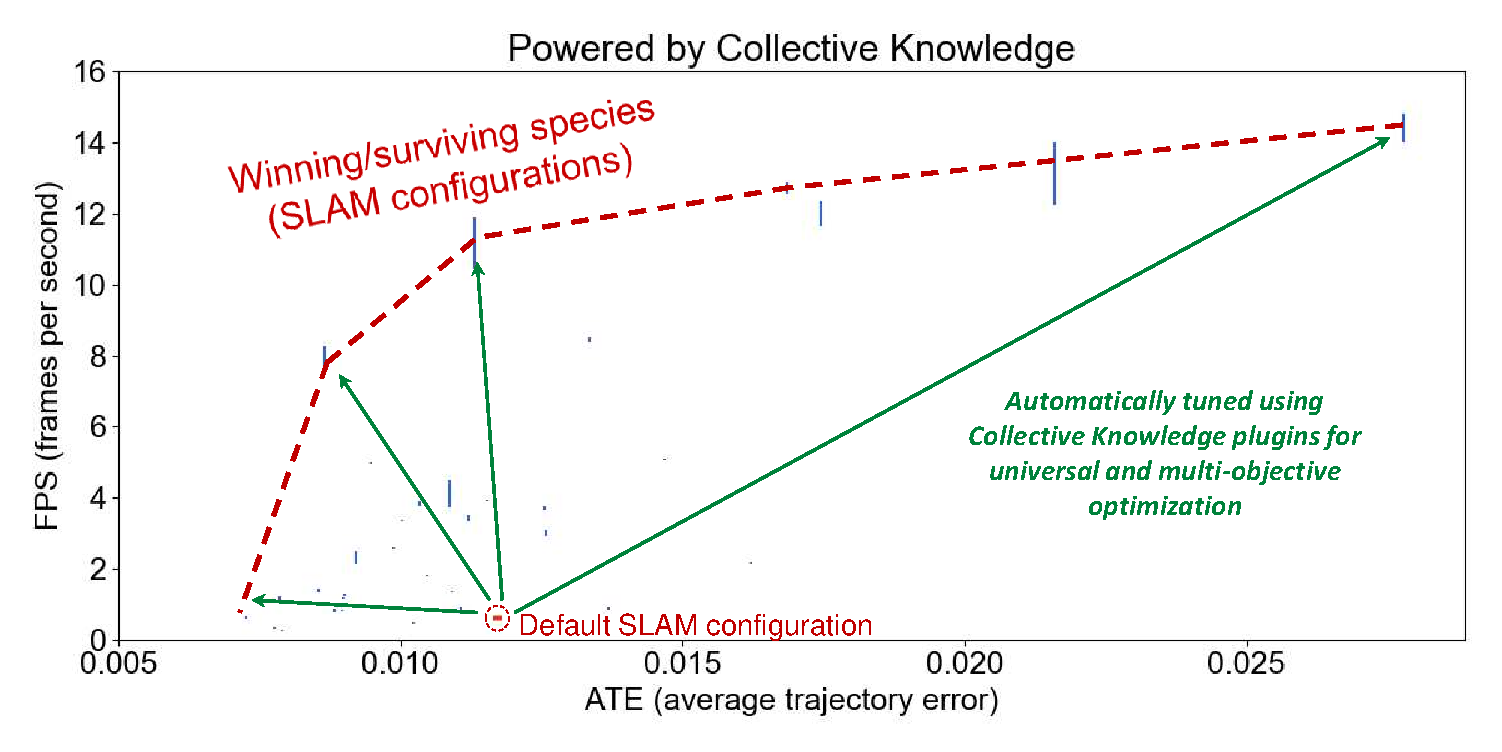
\includegraphics[width=5.8in]
      {ck-assets/37f1624d4b8b53d6-cropped.pdf} %CK_URL={37f1624d4b8b53d6-cropped.pdf}
     \caption{
      Random exploration of various SLAM algorithms and their parameters (Simultaneous localization and mapping)
      in terms of accuracy (average trajectory error or ATE) versus speed 
      (frames per second) on RPi3 using CK.
     }                                         
     \label{fig:converting-ad-hoc-slambench-to-ck}
   \end{figure*}

   %CK={"action":"prepare_for_latex", "cid":"slide:dfd6434297ca601f", "file":"994e7359d7760ab1-cropped.pdf", "path":"ck-assets", "ck_image":"yes", "ck_image_width":700}
   \begin{figure*}[!htbp]
     \centering
      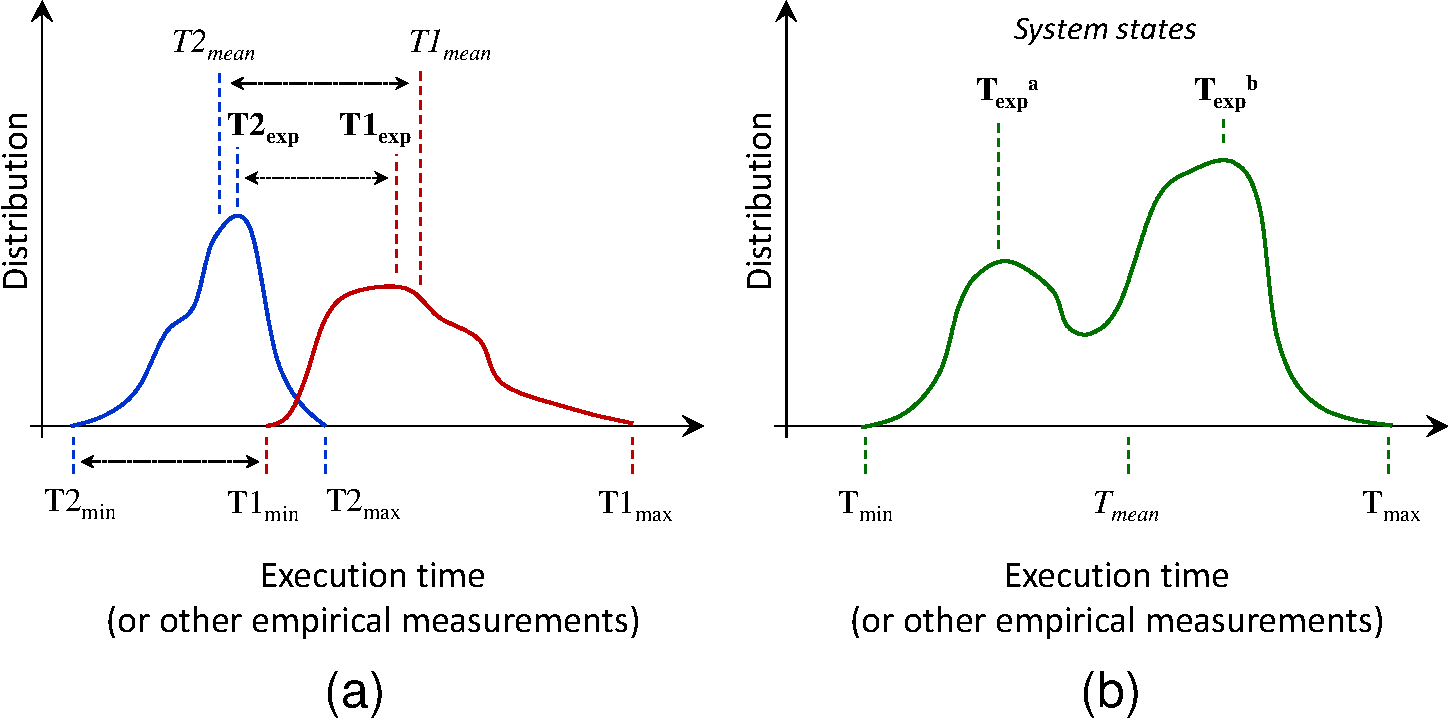
\includegraphics[width=5in]
      {ck-assets/994e7359d7760ab1-cropped.pdf} %CK_URL={994e7359d7760ab1-cropped.pdf}
     \caption{
       Developing common evaluation methodology for empirical results in systems research:
       (a) Calculating speedups between two optimizations T1 and T2 using min, mean and expected values, and reporting max difference.
       (b) Reporting a problem when several system states are detected
     }
     \label{fig:reproducibility}
   \end{figure*}

For a proof-of-concept, we started helping some authors convert their 
artifacts and experimental workflows to the CK format during 
Artifact Evaluation~\cite{ck-shared-repos,Ainsworth:2017:SPI:3049832.3049865,ctuning-ae1}.
%
Association for Computing Machinery (ACM)~\cite{acm} 
also recently joined this effort funded by the Alfred P. Sloan Foundation 
to convert already published experimental workflows 
and artifacs from the ACM Digital Library 
to the CK format~\cite{Flick:2015:PCA:2807591.2807619}.

We can then reuse CK functionality to crowdsource benchmarking and multi-objective
autotuning of shared workloads across diverse data sets, models and platforms.
%
For example, Figure~\ref{fig:converting-ad-hoc-slambench-to-ck} shows 
results from random exploration of various SLAM algorithms (Simultaneous localization and mapping)
and their parameters from~\cite{slambench_paper} in terms of accuracy (average trajectory error or ATE)
versus speed (frames per second) on RPi3 using CK~\cite{ck-slambench-repo}. 
%
Researchers may easily spend 50\% of their time developing
experimental, benchmarking and autotuning infrastructure 
in such complex projects, and then continuously
updating it to adapt to ever changing software and hardware
instead of innovating.
%
Worse, such ad-hoc infrastructure may not even survive 
the end of the project or if leading developers leave project.

Using common and portable workflow framework can relieve researchers
from this burden and let them reuse already existing artifacts and
focus on innovation rather than re-developing ad-hoc software from scratch.
%
Other researchers can also pick up the winning designs on a Pareto frontier,
reproduce results via CK, try them on different platforms
and with different data sets, build upon them, 
and eventually try to develop more efficient algorithms.
%
Finally, researchers can implement a common experimental methodology 
to evaluate empirical results in systems research similar to physics 
within a common workflow framework rather than writing their own
ad-hoc scripts.
%
Figure~\ref{fig:reproducibility} shows statistical analysis 
of experimental results implemented in the CK to compare different
optimizations depending on research scenarios.
%
For example, we report minimal execution time from multiple experiments
to understand the limits of a given architecture, expected value to see
how a given workload performs on average, and max time to detect
abnormal behavior.
%
If more than one expected value is detected, it usually means
that system was in several different run-time states during experiments
(often related to adaptive changes in CPU and GPU frequency due to DVFS)
and extra analysis is required.

%CK={"action":"prepare_for_latex", "cid":"slide:8e550a5184760aab", "file":"b4b07ad3a7839327-cropped.pdf", "path":"ck-assets", "ck_image":"yes", "ck_image_width":600}
\begin{figure*}[!htbp]
  \centering
   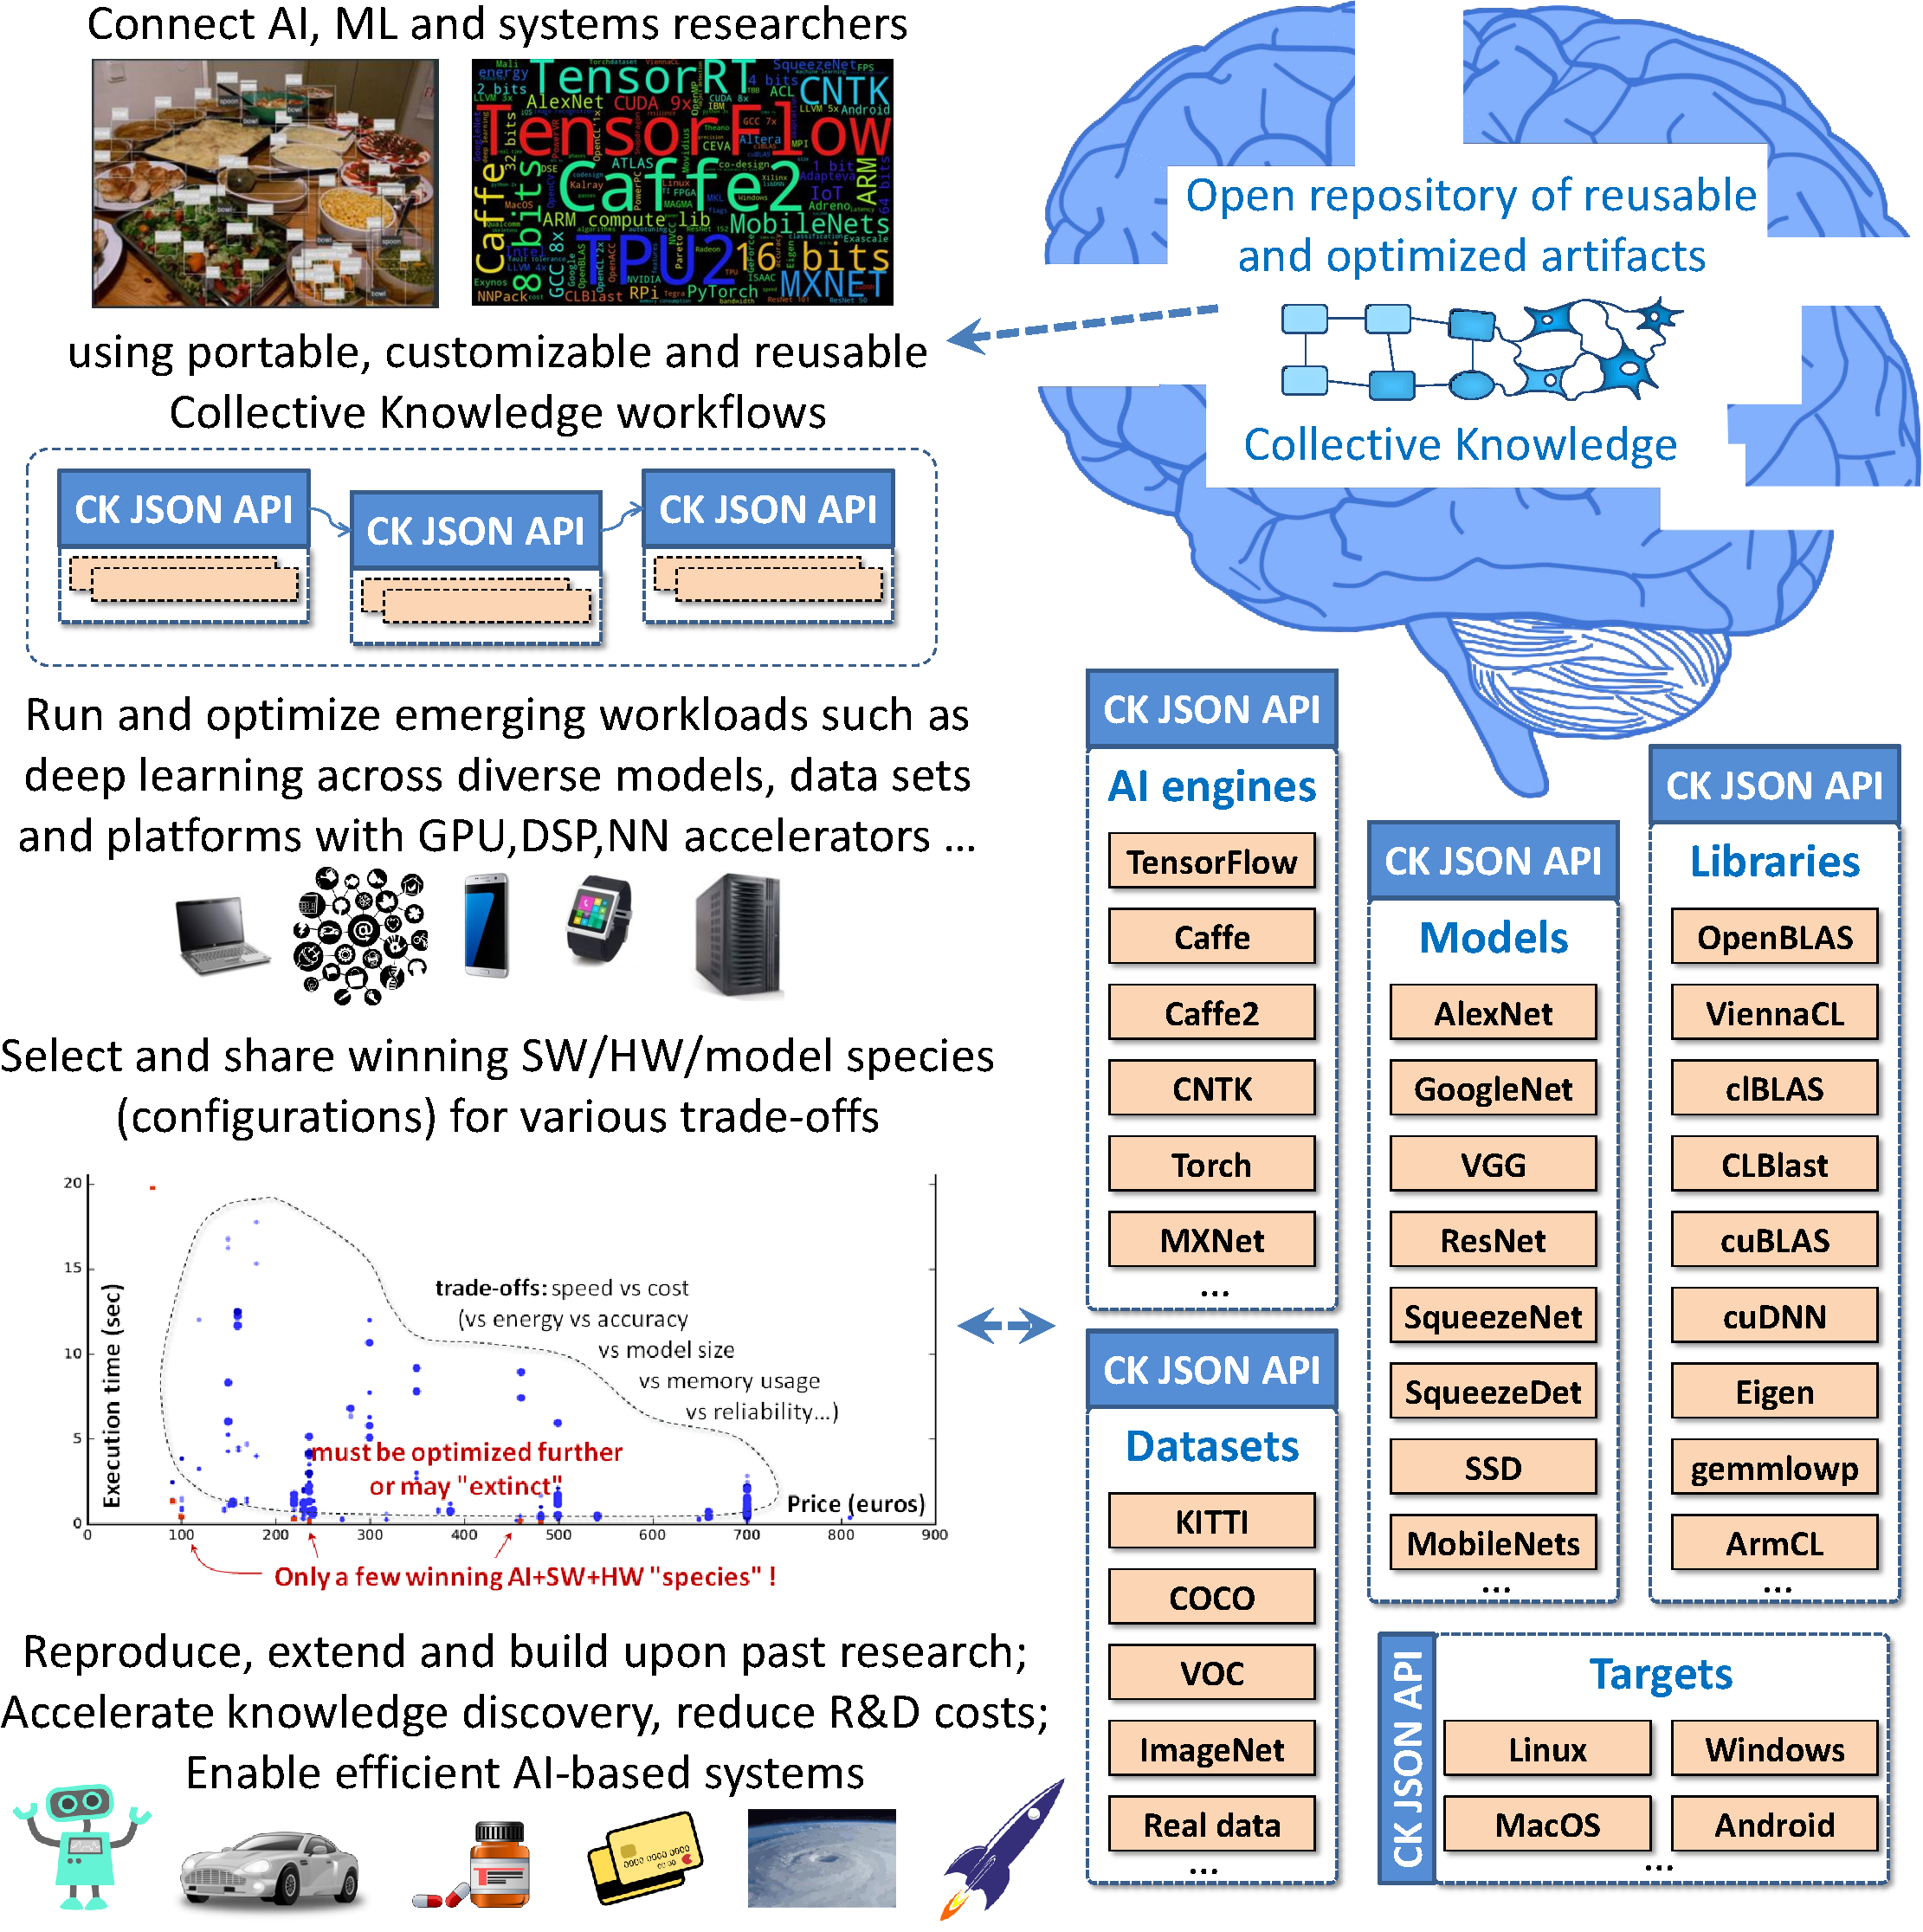
\includegraphics[width=4.5in]
   {ck-assets/b4b07ad3a7839327-cropped.pdf} %CK_URL={b4b07ad3a7839327-cropped.pdf}
  \caption{
    Collective Knowledge framework as an open platform to support software/hardware/model
    co-design tournaments for Pareto-efficient deep learning
    and other emerging workloads in terms of speed, accuracy, 
    energy and various costs.
  }
  \label{fig:reproducible-tournaments}
\end{figure*}

We now plan to validate our Collective Knowledge approach
in the 1st reproducible ReQuEST tournament 
at the ACM ASPLOS'18 conference~\cite{request}
as presented in Figure~\ref{fig:reproducible-tournaments}.
%
ReQuEST is aimed at providing a scalable tournament framework, 
a common experimental methodology and an open repository for continuous evaluation 
and optimization of the quality vs.\ efficiency Pareto optimality of a wide range 
of real-world applications, libraries, and models across the whole 
hardware/software stack on complete platforms. 
%
ReQuEST also promote reproducibility of experimental results and reusability/customization 
of systems research artifacts by standardizing evaluation methodologies and facilitating 
the deployment of efficient solutions on heterogeneous platforms. 

   %CK={"action":"prepare_for_latex", "cid":"slide:4f624e118686001b", "file":"32c0b60dcc114aa8-cropped.pdf", "path":"ck-assets", "ck_image":"yes", "ck_image_width":800}
   \begin{figure*}[!htbp]
     \centering
      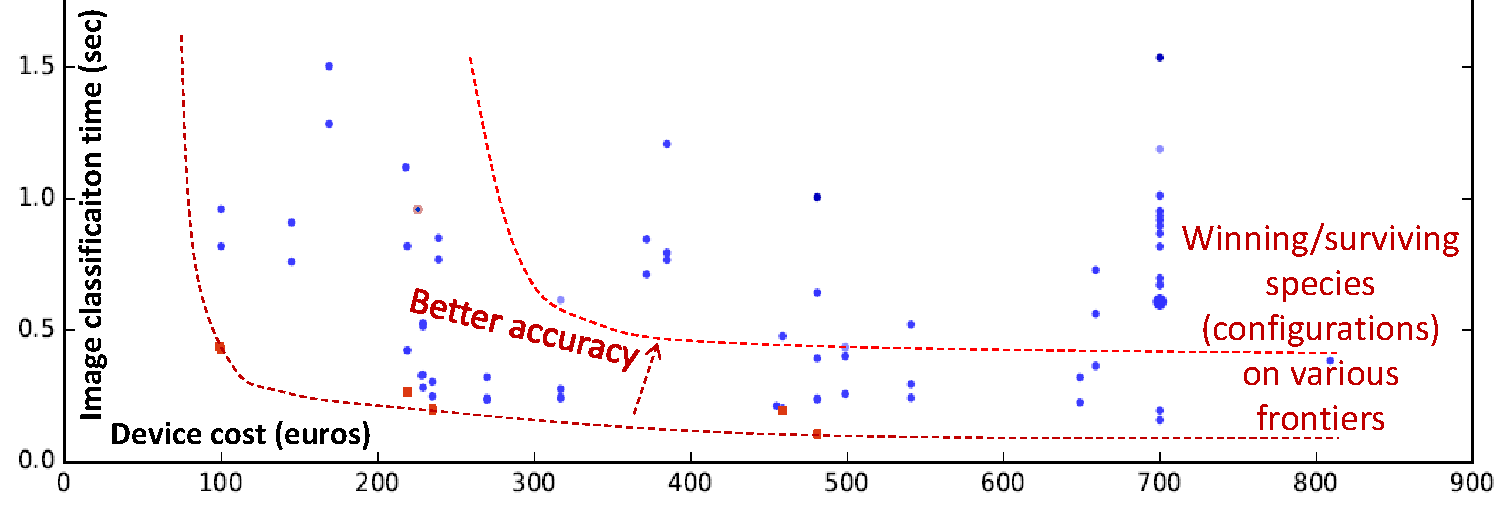
\includegraphics[width=5in]
      {ck-assets/32c0b60dcc114aa8-cropped.pdf} %CK_URL={32c0b60dcc114aa8-cropped.pdf}
     %CK_INTERACTIVE_GRAPH_PASSIVE={"cid":"2d41f89bcf32d4d4:073216ac9e4b4ebc", "where":"div#ck_interactive_f908ef94852bfc65", "html":"interactive.html", "style":"interactive.style", "add_div":"yes", "add_box":"yes", "box_width":800, "remove_script_src":"yes", "remove_script_src":"no"}
     \caption{
      An example of a live Collective Knowledge scoreboard to crowd-benchmark
      inference in terms of speed, accuracy and platform cost 
      across diverse deep learning frameworks, models, data sets, and 
      Android devices provided by volunteers. Red dots 
      are associated with the winning workflows (model/software/hardware)
      on different frontiers.
     }
     \vspace{-1em}
     \label{fig:dnn-crowdtuning-example}
   \end{figure*}

ReQuEST will use CK and our artifact evaluation methodology~\cite{ctuning-ae1} 
to provide unified evaluation and a live scoreboard of submissions. 
%
Figure~\ref{fig:dnn-crowdtuning-example} shows a proof-of-concept example of such a
scoreboard powered by CK to collaboratively benchmark inference (speed vs.\ platform cost) 
across diverse deep learning frameworks (TensorFlow, Caffe, MXNet, etc.), 
models (AlexNet, GoogleNet, SqueezeNet, ResNet, etc.), real user data sets, and mobile devices 
provided by volunteers (see the latest results at \href{http://cknowledge.org/repo}{cKnowledge.org/repo}).
%
Our goal is to teach students and researchers how to 
\begin{itemize}
  \item release research artifacts of their on-going or accomplished research
as portable and reusable components, standardize evaluation workflows, 
and facilitate deployment and tech transfer of state-of-the-art research,
  \item continuously optimize various algorithms
across diverse models, data sets and platforms in terms of speed, accuracy,
size, energy usage and other costs,
  \item build upon each others' work to develop next generation 
of efficient software and hardware stack for emerging workloads.
\end{itemize}

